\documentclass[11pt]{article}

%\usepackage{xcolor} 
\usepackage{amssymb,amsfonts,amsmath,mathrsfs,mathtools}
\usepackage{graphicx, epsfig, epstopdf}
\usepackage{bm}
\usepackage[margin=1in,papersize={8.5in,11in}]{geometry}
\usepackage{times}
\usepackage{xcolor}
\usepackage{color}
\usepackage[pdftex, plainpages=false, colorlinks=true, linkcolor=blue, citecolor=blue, bookmarks=false]{hyperref}
\renewcommand{\thefootnote}{\fnsymbol{footnote}}

\newcommand{\vs}{\vspace{0.2cm}}
\newcommand{\noter}[1]{\textcolor{red}{{#1}}}
\newcommand{\noteb}[1]{\textcolor{blue}{{#1}}}

\makeatother

\def\hs{\hspace{1cm}}

\renewcommand{\baselinestretch}{1.4}

\title{Homework 2}
\author{Gomez - Math 19B}
\date{Due: Jan 26th, 2024}

\begin{document}

\maketitle

\noindent 
\normalsize

Exercises are taken from section 5.2 and 5.3 in the textbook.


\begin{enumerate}

\item 
5.2 Exercise 2: Draw a graph of the signed area represented by the integral and compute it using geometry. 
\[
\int_{-2}^{3} 2x + 4 dx
\]

\item 
5.2 Exercise 12: Calculate $\int_2^52x+1 dx$ in two ways: As the limit $\lim_{N\to\infty} R_N$ and using geometry.

\item 
5.2 Exercise 14: Refer to figure 15, Evaluate $\int_0^3 g(t) dt$ and $\int_3^5 g(t) dt$. 

\begin{center}
    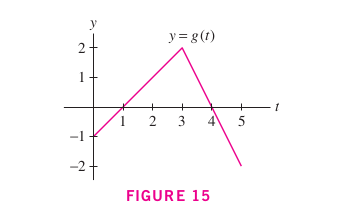
\includegraphics[width=.5\textwidth]{Files/Sect 5.2 Exercise 14-15.png}
\end{center}

\item 
5.2 Exercise 41: Prove by computing the limit of right-endpoint approximations:

\[
\int_0^b x^3 dx = \frac{b^4}{4}
\]

\item 
5.2 Exercise 46: Use the formulas in the summary and equation (9) to evaluate the integral. 

\[
\int_0^1 2x^3 - x + 4 dx
\]
\item 
QUESTION 6
\item 
QUESTION 7
\item 
QUESTION 8
\item 
QUESTION 9


\end{enumerate}
%

%
\end{document}
%
%
